\documentclass{beamer}
\usepackage[orientation=landscape,size=a0,scale=1.4,debug]{beamerposter}
\mode<presentation>{\usetheme{ZH}}
\usepackage{chemformula}
\usepackage{relsize}
\usepackage[font=tiny,labelfont=bf]{caption}
\usepackage{graphics}
\usepackage{booktabs} % Allows the use of \toprule, \midrule and \bottomrule in tables
\usepackage[utf8]{inputenc}
\usepackage[german, english]{babel} % required for rendering German special characters
\usepackage{siunitx} %pretty measurement unit rendering
\usepackage{hyperref} %enable hyperlink for urls
\usepackage{ragged2e}
\usepackage[font=scriptsize,justification=justified]{caption}
\usepackage{array,booktabs,tabularx}
\newcommand{\bigqm}[1][1]{\text{\larger[#1]{\textbf{?}}}}
\newcolumntype{Z}{>{\centering\arraybackslash}X} % centered tabularx columns
\sisetup{per=frac,fraction=sfrac}

\title{\huge A Distributed and Parallel Asynchronous Unite and Conquer Method to Solve Non-Hermitian Linear Systems}
\author{Xinzhe WU$^{1,2}$, Serge G. Petiton$^{1,2}}
\institute[ETH]{$^{1}$Maison de La Simulation, CNRS UMR 3441, 91191, Gif sur Yvette, France \\ $^{2}$Centre de Recherche en Informatique, Signal et Automatique de Lille (CRIStAL), CNRS UMR 9189, Universit\'e de Lille 1, Sciences et Technologies, 59655 Villeneuve d'Ascq Cedex, France}
\date{\today}

% edit this depending on how tall your header is. We should make this scaling automatic :-/
\newlength{\columnheight}
\setlength{\columnheight}{104cm}

\begin{document}
\begin{frame}
\vspace{0.45em}
\begin{columns}
	\begin{column}{.33\textwidth}
		\begin{beamercolorbox}[center]{postercolumn}
			\begin{minipage}{.98\textwidth}  % tweaks the width, makes a new \textwidth
				\parbox[t][\columnheight]{\textwidth}{ % must be some better way to set the the height, width and textwidth simultaneously
					\begin{myblock}{Background}
						\begin{itemize}
							\item Linear Systems Solvers
							\begin{figure}[H]
              				\centering
             				\includegraphics[width=0.74\linewidth]{img/linear_systems2.png}
              				\end{figure}
							\item SuperComputing and Parallel Programming Trends
							\begin{itemize}
                				\item Highly hierarchical architectures (Computing and Memeory)
                				\item Increasing levels and degree of parallelism
                				\item Heterogeneity (Computing, Memory and Scalability)
                			\end{itemize}
                			\vspace{0.5cm}
                		\item Requirement of parallel programming
						\begin{itemize}
							\item Multi-grain, multi-level memory
							\item Reducing synchronizations and promoting asynchronicity
							\item Multi-level scheduling strategies
						\end{itemize}
						\end{itemize}
						\vspace{0.4em}
					\end{myblock}
					\begin{myblock}{Krylov Subspace Methods}
					\vspace{0.4em}
					\begin{figure}
							\begin{minipage}{.72\textwidth}
								\centering\includegraphics[width=\textwidth]{img/krylov.png}
							\end{minipage}
					\end{figure}
            			\vspace{0.5em}

              		\begin{itemize}
              			\item Non-Hermitian Linear System Slovers
                		\begin{itemize}
                			\item Restarted GMRES
                			\item Deflated GMRES
                			\item Flexible GMRES
                		\end{itemize}
                		\vspace{0.5em}
              			\item Non-Hermitian Eigenvalues Problems Solvers
                		\begin{itemize}
                			\item Explicitly Restarted Arnoldi Method (ERAM)
                			\item Implicitly Restarted Arnoldi Method (IRAM)
                		\end{itemize}
              		\end{itemize}  
						\vspace{0.5em}
						\begin{figure}
							\begin{minipage}{1.01\textwidth}
								\centering\includegraphics[width=0.9\textwidth]{img/gmres.png}
								\caption{Basic Restarted GMRES Method.}
								\label{fig:stim}
							\end{minipage}
						\end{figure}
						\vspace{0.5em}
						{\color{red}$\bigqm[6]$}
						          \large The improvement is intrinsic to the method.
How to design a method which allows the improvement from one time resolution to another?
					\end{myblock}\vfill
		}\end{minipage}\end{beamercolorbox}
	\end{column}

	\begin{column}{.33\textwidth}
		\begin{beamercolorbox}[center]{postercolumn}
			\begin{minipage}{.98\textwidth} % tweaks the width, makes a new \textwidth
				\parbox[t][\columnheight]{\textwidth}{ % must be some better way to set the the height, width and textwidth simultaneously
					\begin{myblock}{Least Squares Polynomial Method}
					Iterates: $x_n=x_0+P_n(A)r_0$ \rightarrow $r_n=R_n(A)r_0$, with $R_n(\lambda)=1-\lambda P_n(\lambda)$. 
					The purpose is to find a kind of polynomial $P_n$ which can minimize $R_n(A)r_0$. For more details of this method, see the article \cite{saad1987least}.

					\vspace{.3em}
					\begin{figure}
							\begin{minipage}{.60\textwidth}
								\centering\includegraphics[width=\textwidth]{img/residu.png}
							\end{minipage}
					\end{figure}

						\begin{figure}
							\begin{minipage}{0.6\textwidth}
								\centering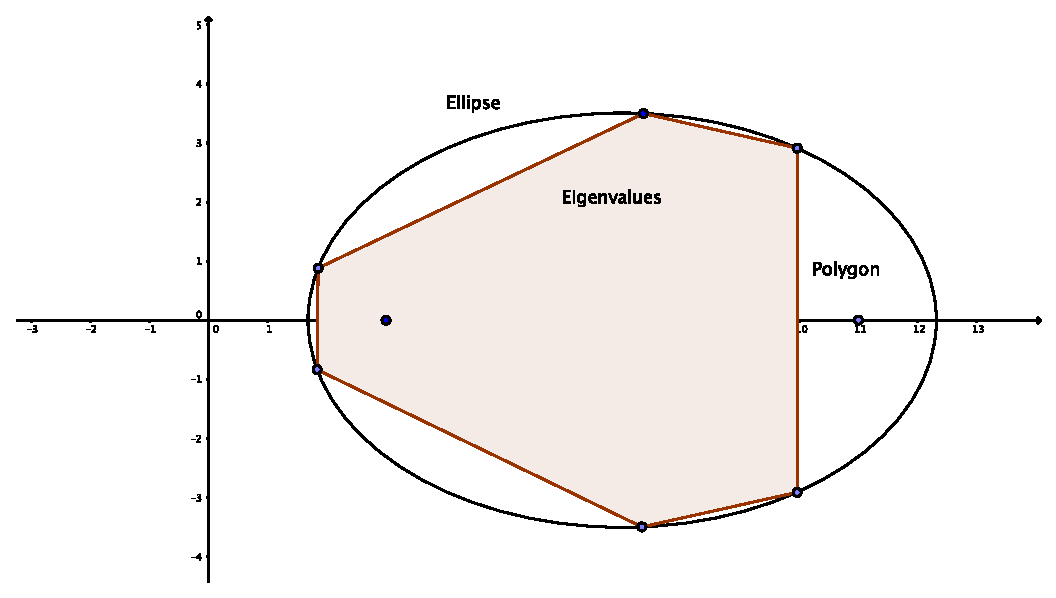
\includegraphics[width=0.6\textwidth]{img/polygon.eps}
								\caption{Eigenvalues, convex hull and ellipse.}
								\label{fig:fail}
							\end{minipage}
							\hspace{0.6em}
							\begin{minipage}{0.31\textwidth}
								\centering\includegraphics[width=0.44\textwidth]{img/lsqr.png}
								\caption{Least Squares Polynomial Preconditioner.}
								\label{fig:fail}
							\end{minipage}
						\end{figure}
					\end{myblock}

					\begin{myblock}{UCGLE Method}
						UCGLE: Unite and Conquer \cite{emad2016unite} GMRES-LS/ERAM method
						\vspace{0.6em}
						\begin{figure}
							\begin{minipage}{.5\textwidth}
								\centering\includegraphics[width=\textwidth]{img/glsa_mpi.png}
								\caption{UCGLE Method Workflow}
							\end{minipage}
						\end{figure}
					\end{myblock}


					\begin{myblock}{Implementation}
				UCGLE is implemented using the libraries PETSc and SLEPc, was successfully installed on ROMEO in Reims, France, and on Tianhe-2 (6 times No.1 and now No.2 in Top500 List) in Guangzhou, China.
\vspace{0.5em}

\begin{table}[!t]
\footnotesize
\renewcommand{\arraystretch}{1.3}
%\newcommand{\tabincell}[2]{\begin{tabular}{@{}#1@{}}#2\end{tabular}}  
\label{table3}
\centering
\begin{tabular}{|c|c|c|}
\hline
Plateforms: &Tianhe-2 &ROMEO \\
\hline
Speed (LINPACK) & 33,862.7 TFlop/s & 254.9 TFlop/s\\
\hline
Power & 17,808.00 kW & 81.41 kW\\
\hline
Architectures & \begin{tabular}{@{}c@{}} 3,120,000 Intel Xeon \\ E5-2692v2 12C 2.2GHz\end{tabular} &\begin{tabular}{@{}c@{}} 5, 720 Intel Xeon \\ E5-2650v2 8C 2.6GHz\end{tabular}\\
\hline
\end{tabular}
%\caption{Specifications of Tianhe-2 in National Supercomputer Center in Guangzhou, China}
\end{table}

					\end{myblock}


		}\end{minipage}\end{beamercolorbox}
	\end{column}
\begin{column}{.33\textwidth}
		\begin{beamercolorbox}[center]{postercolumn}
			\begin{minipage}{.98\textwidth}  % tweaks the width, makes a new \textwidth
				\parbox[t][\columnheight]{\textwidth}{ % must be some better way to set the the height, width and textwidth simultaneously

					\begin{myblock}{Experimental Results}
					Convergence Comparison and Performance Comparison \cite{xwu2017}:
						\begin{figure}
							\begin{minipage}{0.84\textwidth}
								\centering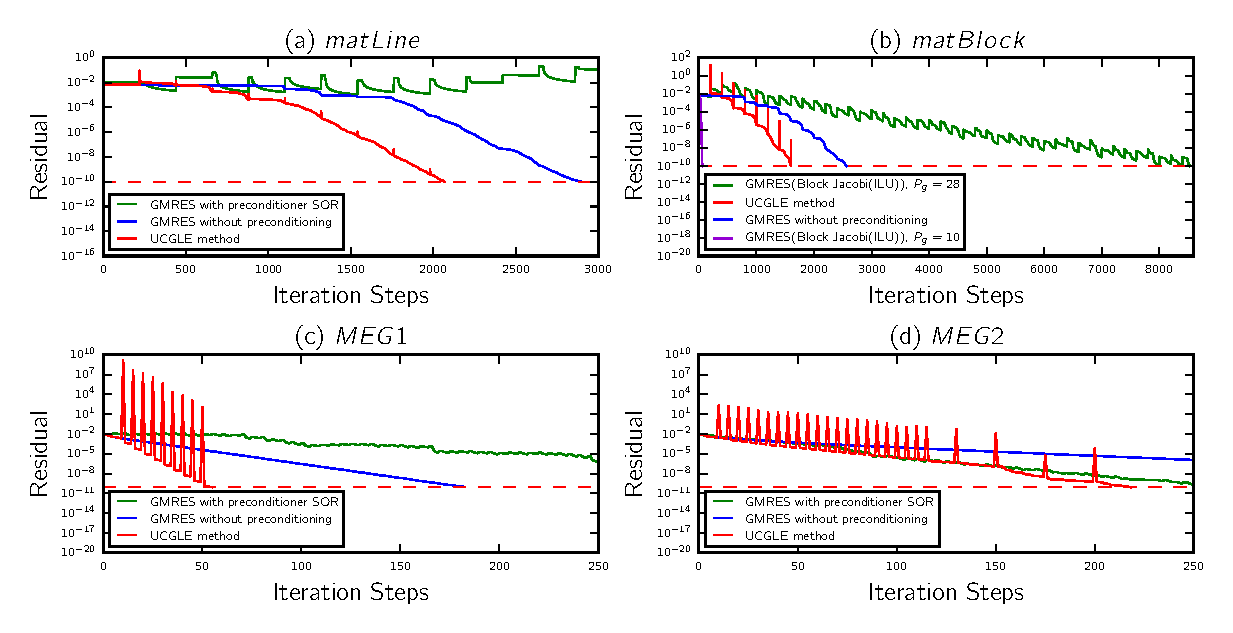
\includegraphics[width=1\textwidth, height=0.2\textheight]{img/convergence.eps}
								\caption{Convergence analysis of UCGLE method, traditional restarted GMRES and GMRES with different preconditioners.}
							\end{minipage}
						\end{figure}
						\begin{figure}
							\begin{minipage}{0.82\textwidth}
								\centering\includegraphics[width=1\textwidth,height=0.1\textheight]{img/performance_time.eps}
								\caption{Convergence time of UCGLE, with the sum of GMRES Component process number and ERAM Component process number fixed}
							\end{minipage}
						\end{figure}

					\end{myblock}

					\begin{myblock}{Summary and Perspective}
This poster outlines a distributed and parallel method UCGLE for the resolution of non-Hermitian linear systems to explore the novel numerical parallel methods. \\
\vspace{0.1em}
In future, there are still lots of aspects to evaluate. Firstly, we should study the the impacts of different parameters of each component on the performance of UCGLE. Secondly, it’s necessary to study the influence of the eigenvalues on UCGLE, and summarize the scenes suited to this method. In the end, we plan to implement this method based on the workflow and distributed parallel methodologies YML-XMP, a kind of user-friendly and hierarchical-system-oriented development and execution environment.

					\end{myblock}


					\begin{myblock}{References}
						\footnotesize
						\bibliographystyle{abbrv}
						\bibliography{./bib}
					\end{myblock}

		}\end{minipage}\end{beamercolorbox}
	\end{column}
\end{columns}
\end{frame}
\end{document}
